\documentclass[11pt]{article}

\usepackage[utf8]{inputenc}
\usepackage[margin=1in]{geometry}
\usepackage[english]{babel}
\usepackage{tocloft}
\usepackage{amsmath}
\usepackage{amsfonts}
\usepackage{amssymb}
\usepackage[none]{hyphenat}
\usepackage{graphicx}
\usepackage{fancyhdr}
\usepackage{pdfpages}
\usepackage[font={small,it}]{caption}

\parindent 0ex
\linespread{1.5}
\setlength{\headheight}{30pt}
\setcounter{tocdepth}{1}
\pagestyle{fancy}

\fancyhead{}
%\fancyfoot{}
\fancyhead[L]{\slshape \MakeUppercase{Cryptogen User Manual}}
\rhead{
\includegraphics[width=1.5cm, height=1.5cm]{cryogen.png}
\includegraphics[width=1.5cm, height=1.5cm]{icon.png}}

\begin{document}
	%insert pdf cover page
	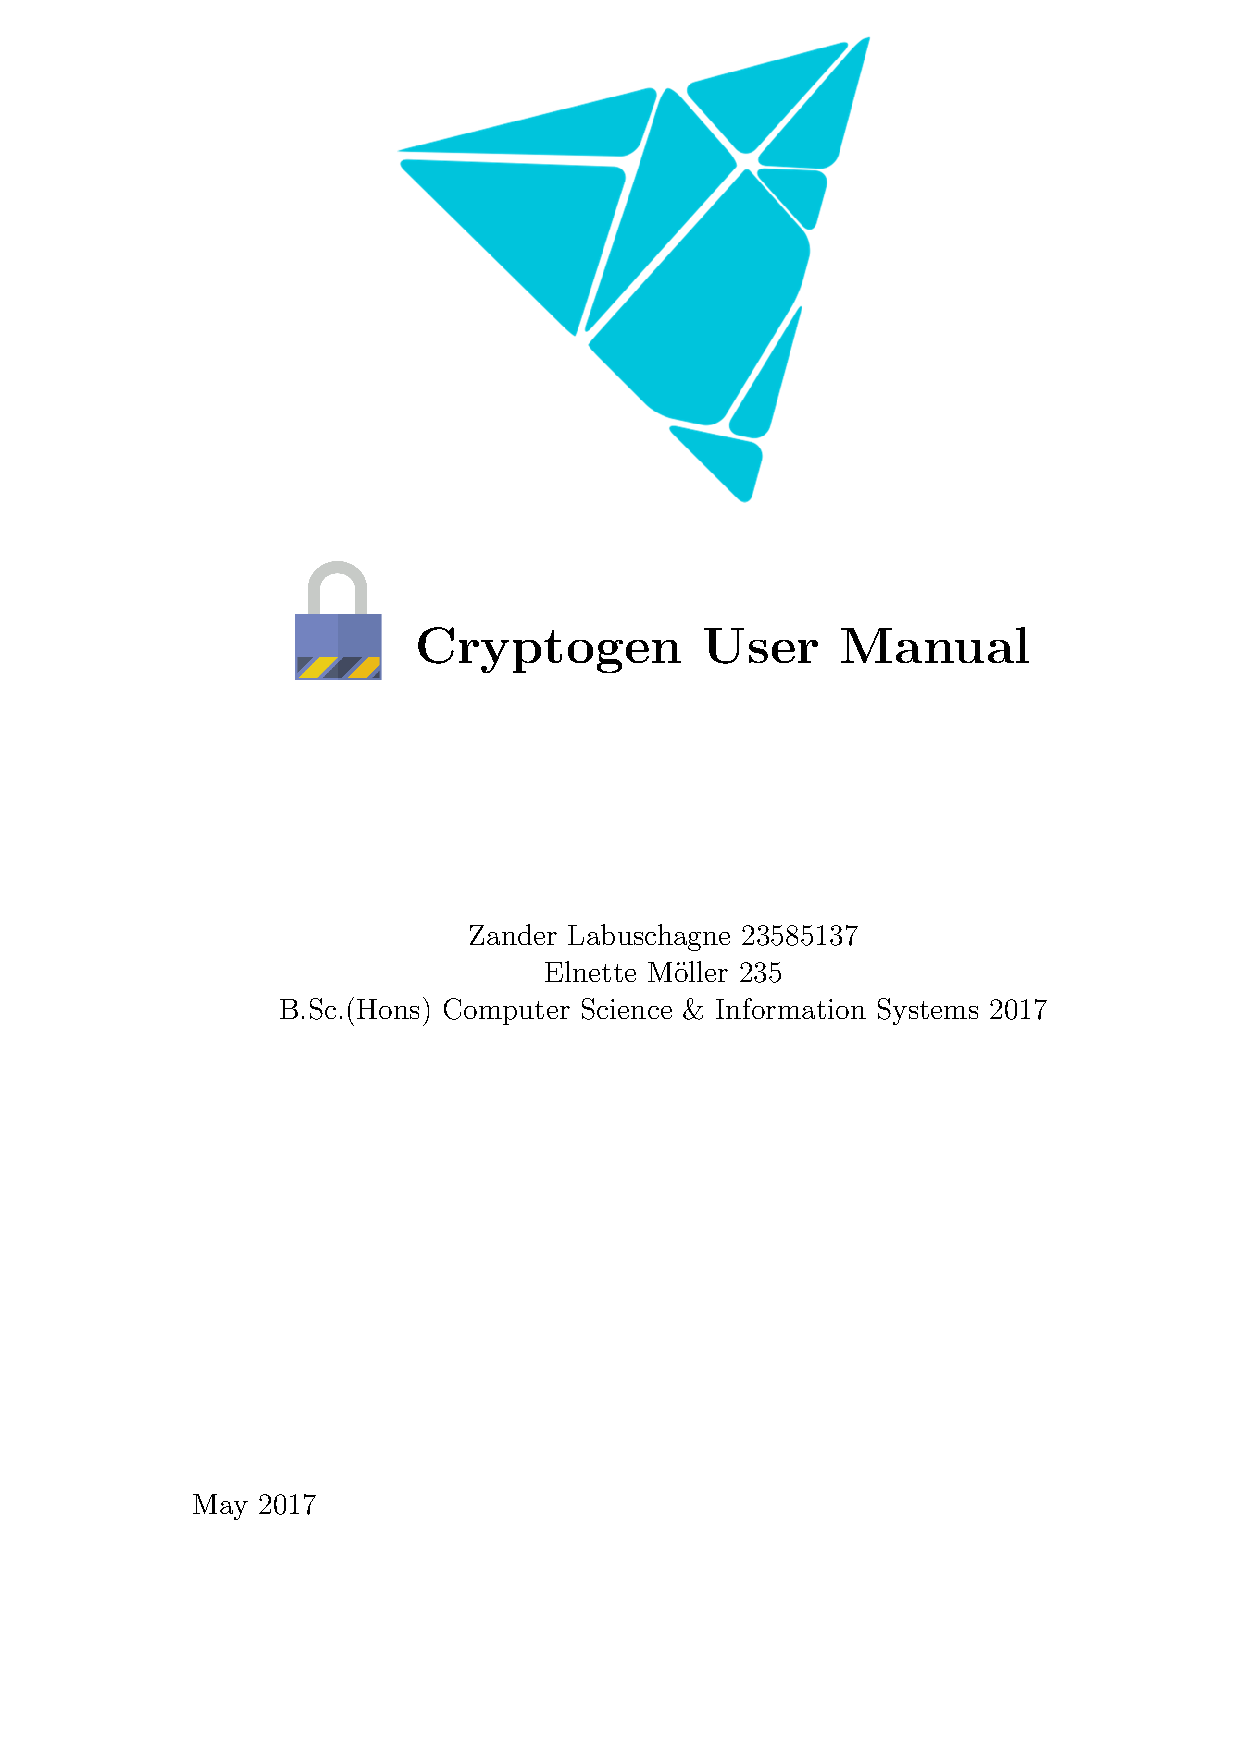
\includepdf[pages={-},offset=0mm 0mm, width=21.5cm, height=28cm]{Cover.pdf}

    \renewcommand{\cftsecleader}{\cftdotfill{\cftdotsep}} % TOC Dotted Lines
    \tableofcontents
    \thispagestyle{empty}
    \clearpage

	%\printglossary[title=Abbreviation]

    \setcounter{page}{1}

	\section{Introduction} % 1-2p[0.5p] : Agtergrond : Rationale
		...



    	\section{Reflection}
		...

    \newpage
    \bibliographystyle{plain}
    \bibliography{ref}
    \addcontentsline{toc}{section}{{}References}
    \thispagestyle{plain}
    \clearpage

  %  \section*{Appendix A: Research Proposal}
  %  \addcontentsline{toc}{section}{{}Appendix A: Research Proposal}
    %\pagenumbering{gobble}
  %  \includepdf[pages={-},offset=0mm 0mm, width=21.5cm, height=28cm]{Appendix_A.pdf}

\end{document}
